% Source-SHA256: 11e53403d4d2c43a9d86b8ed516fa36893003dc083ac9525fa113a292d6ef807
% !TeX program = xelatex
\documentclass[a4paper,11pt]{article}
\usepackage{fontspec}
\IfFontExistsTF{TeX Gyre Pagella}{\setmainfont{TeX Gyre Pagella}}{\setmainfont{P052}}
\IfFontExistsTF{TeX Gyre Heros}{\setsansfont{TeX Gyre Heros}}{\setsansfont{Nimbus Sans}}
\IfFontExistsTF{TeX Gyre Cursor}{\setmonofont{TeX Gyre Cursor}[Scale=0.88]}{\setmonofont{Nimbus Mono PS}[Scale=0.88]}
\usepackage{babel}
\babelprovide[import,main]{spanish}
\usepackage{microtype}
\usepackage[a4paper,margin=2.4cm,headheight=23pt,headsep=10pt,footskip=1.1cm]{geometry}
\raggedbottom
\setlength{\emergencystretch}{3em}
\hyphenpenalty=10000
\exhyphenpenalty=10000
\clubpenalty=10000
\widowpenalty=10000
\usepackage{xcolor}
\definecolor{navybg}{HTML}{0B1D2E}
\definecolor{navydeep}{HTML}{123049}
\definecolor{lightblue}{HTML}{8FD3FE}
\definecolor{amber}{HTML}{F5A623}
\definecolor{softgray}{HTML}{5B6570}
\usepackage{titlesec,needspace}
\setcounter{secnumdepth}{-1}
\setcounter{tocdepth}{2}
\titleformat{\section}{\sffamily\Large\bfseries\color{navydeep}\raggedright}{}{0pt}{}
\titleformat{\subsection}{\sffamily\large\bfseries\color{navydeep}\raggedright}{}{0pt}{}
\titlespacing*{\section}{0pt}{20pt}{9pt}
\titlespacing*{\subsection}{0pt}{14pt}{6pt}
\usepackage{fancyhdr}
\pagestyle{fancy}
\fancyhf{}
\fancyhead[L]{\small\sffamily\color{softgray}Compás a compás}
\fancyhead[R]{\small\sffamily\color{softgray}Instalación y arranque}
\fancyfoot[L]{\small\sffamily\color{softgray}Aplicación 0.6.0 · 17/10/2026}
\fancyfoot[R]{\small\sffamily\color{softgray}\thepage}
\renewcommand{\headrulewidth}{0.4pt}
\usepackage{array,longtable,booktabs,calc}
\newcounter{none}
\renewcommand{\arraystretch}{1.15}
\usepackage{enumitem}
\setlist[itemize]{leftmargin=1.4em,itemsep=3pt,topsep=5pt}
\setlist[enumerate]{leftmargin=1.8em,itemsep=3pt,topsep=5pt}
\usepackage{fvextra,framed,seqsplit}
\fvset{fontsize=\small,breaklines=true,breakanywhere=true,frame=leftline,framerule=1.4pt,rulecolor=\color{lightblue},framesep=8pt}
\RecustomVerbatimEnvironment{verbatim}{Verbatim}{breaklines,breakanywhere,samepage=true,fontsize=\small}
\let\originaltexttt\texttt
\renewcommand{\texttt}[1]{\originaltexttt{\seqsplit{#1}}}
\providecommand{\tightlist}{\setlength{\itemsep}{2pt}\setlength{\parskip}{0pt}}
\usepackage{graphicx,xurl,tikz}
\usepackage[section]{placeins}
\usepackage{amssymb,newunicodechar}
\usepackage[colorlinks=true,linkcolor=navydeep,urlcolor=navydeep,pdftitle={Compás a compás - Instalación y arranque},pdfauthor={Jesús Quevedo Rodríguez}]{hyperref}
\usepackage{bookmark}
\newunicodechar{♭}{\texorpdfstring{\ensuremath{\flat}}{\unichar{9837}}}
\newunicodechar{♯}{\texorpdfstring{\ensuremath{\sharp}}{\unichar{9839}}}
\newunicodechar{✓}{\texorpdfstring{\ensuremath{\checkmark}}{\unichar{10003}}}
\newunicodechar{✗}{\texorpdfstring{\ensuremath{\times}}{\unichar{10007}}}
\newunicodechar{→}{\texorpdfstring{\ensuremath{\rightarrow}}{\unichar{8594}}}
\newunicodechar{←}{\texorpdfstring{\ensuremath{\leftarrow}}{\unichar{8592}}}
\setlength{\parindent}{0pt}
\setlength{\parskip}{6pt}
\renewcommand{\topfraction}{0.95}
\renewcommand{\bottomfraction}{0.95}
\renewcommand{\textfraction}{0.05}
\renewcommand{\floatpagefraction}{0.6}
\setcounter{topnumber}{3}
\setcounter{totalnumber}{4}
\begin{document}
\begin{titlepage}
\newgeometry{margin=0cm}
\thispagestyle{empty}
\pagecolor{navybg}
\color{white}
\vspace*{3cm}
\begin{center}
{\sffamily\bfseries\fontsize{16}{19}\selectfont\color{amber} COMPÁS A COMPÁS\par}
\vspace{1cm}
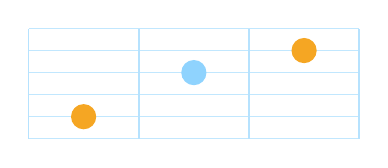
\begin{tikzpicture}[x=0.7cm,y=0.28cm]
\foreach \y in {0,...,5} {\draw[lightblue!55,line width=0.5pt] (-3,\y)--(3,\y);}
\foreach \x in {-3,-1,1,3} {\draw[lightblue!65,line width=0.6pt] (\x,0)--(\x,5);}
\fill[amber] (-2,1) circle[x radius=0.16cm,y radius=0.16cm];
\fill[lightblue] (0,3) circle[x radius=0.16cm,y radius=0.16cm];
\fill[amber] (2,4) circle[x radius=0.16cm,y radius=0.16cm];
\end{tikzpicture}\par
\vspace{1.4cm}
{\sffamily\bfseries\fontsize{30}{38}\selectfont Instalación y arranque\par}
\vspace{0.8cm}
{\sffamily\fontsize{14}{20}\selectfont\color{lightblue} Abrir la aplicación desde la carpeta del proyecto\par}
\vfill
{\sffamily\small Autor del proyecto: Jesús Quevedo Rodríguez\par}
{\sffamily\small Aplicación 0.6.0 · 17/10/2026\par}
{\sffamily\small Repositorio: a01653/Compas-a-compas\par}
\vspace{2cm}
\end{center}
\end{titlepage}
\nopagecolor
\restoregeometry
\setcounter{page}{2}
\tableofcontents
\newpage
Aplicación 0.6.0 · Edición del manual: 17/10/2026. Autor del proyecto:
Jesús Quevedo Rodríguez.

\Needspace{3.5cm}
\hypertarget{quuxe9-necesitas}{%
\section{Qué necesitas}\label{quuxe9-necesitas}}

\begin{itemize}
\tightlist
\item
  Windows para el lanzador de doble clic.
\item
  \textbf{Node.js 18 o superior}, con \texttt{node.exe} disponible en el
  PATH.
\item
  Un navegador. Las comprobaciones realizadas usan Chromium.
\item
  La carpeta completa del repositorio. No hay dependencias npm que
  instalar.
\end{itemize}

La aplicación funciona en tu equipo, sin cuentas ni backend. Para usarla
no hacen falta Claude, el conector ni el túnel de Cloudflare. Python,
Pandoc y LaTeX solo se usan si quieres regenerar esta documentación.

\Needspace{3.5cm}
\hypertarget{tener-el-proyecto-en-su-carpeta}{%
\section{Tener el proyecto en su
carpeta}\label{tener-el-proyecto-en-su-carpeta}}

La ruta prevista en este equipo es:

\begin{verbatim}
C:\temp\Compas-a-compas
\end{verbatim}

Si ya tienes el repositorio, actualízalo siguiendo el apartado de
actualización. Si todavía no lo tienes y dispones de Git con acceso al
repositorio, abre PowerShell y ejecuta:

\begin{verbatim}
git clone https://github.com/a01653/Compas-a-compas.git C:\temp\Compas-a-compas
\end{verbatim}

No ejecutes el clonado sobre una carpeta que ya contiene el proyecto. Si
descargas un ZIP, extrae todo su contenido: no basta con copiar
\texttt{index.html}.

En la raíz deben estar \texttt{Abrir-Compas.cmd}, \texttt{index.html},
\texttt{package.json}, \texttt{scripts}, \texttt{src}, \texttt{styles},
\texttt{assets} y \texttt{references}. Los manuales y sus fuentes están
en \texttt{docs}.

\Needspace{3.5cm}
\hypertarget{abrir-cada-duxeda}{%
\section{Abrir cada día}\label{abrir-cada-duxeda}}

\begin{enumerate}
\def\labelenumi{\arabic{enumi}.}
\tightlist
\item
  Abre \texttt{C:\textbackslash{}temp\textbackslash{}Compas-a-compas} en
  el Explorador.
\item
  Haz doble clic en \textbf{Abrir-Compas.cmd}.
\item
  Se abrirá el navegador en \texttt{http://127.0.0.1:5174}.
\item
  Pulsa \textbf{Abrir JSON} y elige tu canción guardada, o acepta la
  recuperación local si se ofrece y corresponde a tu trabajo.
\end{enumerate}

Puedes crear un acceso directo a \texttt{Abrir-Compas.cmd} en el
escritorio. Mantén el archivo original dentro del proyecto.

La consola que arranca el servidor debe permanecer abierta. Al terminar,
guarda tu JSON y pulsa \textbf{Ctrl+C} en esa consola para detenerlo. Si
el servidor ya estaba abierto, el lanzador reutiliza esa instancia y su
segunda ventana puede cerrarse sola; la consola original sigue siendo la
que mantiene la aplicación.

Si sigue abierta una instancia de una carpeta antigua o un
\emph{worktree}, ciérrala antes de arrancar desde la carpeta principal.
El lanzador reconoce la aplicación del puerto 5174 y puede reutilizar
esa instancia anterior.

\Needspace{3.5cm}
\hypertarget{arranque-manual}{%
\section{Arranque manual}\label{arranque-manual}}

Si necesitas ver los mensajes o usar otro puerto:

\begin{verbatim}
cd C:\temp\Compas-a-compas
npm.cmd start
\end{verbatim}

Abre \texttt{http://127.0.0.1:5174}. Para otro puerto:

\begin{verbatim}
npm.cmd start -- --port 8080
\end{verbatim}

En ese caso abre \texttt{http://127.0.0.1:8080}. El lanzador de doble
clic siempre utiliza 5174. En Linux y macOS se usa \texttt{npm\ start}
desde la raíz del proyecto.

El servidor escucha solo en \texttt{127.0.0.1}: es una aplicación local
del equipo. Abrir \texttt{index.html} con doble clic no arranca el
editor; sus módulos necesitan una dirección HTTP. Los HTML exportados sí
pueden abrirse directamente sin servidor.

\Needspace{3.5cm}
\hypertarget{actualizar-sin-perder-las-canciones}{%
\section{Actualizar sin perder las
canciones}\label{actualizar-sin-perder-las-canciones}}

\begin{enumerate}
\def\labelenumi{\arabic{enumi}.}
\tightlist
\item
  Guarda el proyecto abierto como JSON en una carpeta conocida.
\item
  Detén la consola que sirve la aplicación.
\item
  Actualiza la copia principal:
\end{enumerate}

\begin{verbatim}
git -C C:\temp\Compas-a-compas pull --ff-only origin main
\end{verbatim}

\begin{enumerate}
\def\labelenumi{\arabic{enumi}.}
\setcounter{enumi}{3}
\tightlist
\item
  Vuelve a abrir \textbf{Abrir-Compas.cmd} y recarga el navegador con
  \textbf{Ctrl+F5}.
\item
  Comprueba la versión visible y abre tu JSON.
\end{enumerate}

Si Git avisa de cambios locales o de ramas divergentes, detente y revisa
esos cambios antes de continuar. No hace falta borrar carpetas ni
descartar archivos para una actualización normal. Los JSON guardados son
tus copias editables: mantenlos aparte de los archivos de programa.

\Needspace{3.5cm}
\hypertarget{resolver-los-problemas-habituales}{%
\section{Resolver los problemas
habituales}\label{resolver-los-problemas-habituales}}

\begin{longtable}[]{@{}>{\raggedright\arraybackslash}p{\dimexpr0.320000\linewidth-1.000000\tabcolsep\relax}>{\raggedright\arraybackslash}p{\dimexpr0.680000\linewidth-1.000000\tabcolsep\relax}@{}}
\toprule\noalign{}
Mensaje o síntoma & Solución \\
\midrule\noalign{}
\endhead
\bottomrule\noalign{}
\endlastfoot
Falta Node.js o la versión es antigua & Instala o actualiza Node.js a 18
o superior. Reabre la consola y comprueba \texttt{node\ -\/-version}. \\
PowerShell bloquea \texttt{npm.ps1} & Usa el lanzador o escribe
\texttt{npm.cmd\ start}, como en esta guía. \\
El puerto 5174 está ocupado por otra aplicación & No cierres procesos al
azar. Identifica la aplicación o arranca manualmente en otro puerto. \\
El navegador no se abre automáticamente & Conserva la consola y abre a
mano la URL que indica. \\
La página deja de responder & Comprueba que sigue abierta la consola del
servidor y que usas su mismo puerto. \\
Aparece una versión anterior & Cierra la instancia anterior, actualiza
la carpeta principal, arranca otra vez y pulsa Ctrl+F5. \\
No encuentro mi canción al volver & Abre el JSON que guardaste. La
recuperación depende del navegador y del puerto utilizados. \\
\end{longtable}

\Needspace{3.5cm}
\hypertarget{duxf3nde-estuxe1n-la-ayuda-y-los-archivos}{%
\section{Dónde están la ayuda y los
archivos}\label{duxf3nde-estuxe1n-la-ayuda-y-los-archivos}}

\begin{longtable}[]{@{}>{\raggedright\arraybackslash}p{\dimexpr0.320000\linewidth-1.000000\tabcolsep\relax}>{\raggedright\arraybackslash}p{\dimexpr0.680000\linewidth-1.000000\tabcolsep\relax}@{}}
\toprule\noalign{}
Archivo o carpeta & Uso \\
\midrule\noalign{}
\endhead
\bottomrule\noalign{}
\endlastfoot
\texttt{Abrir-Compas.cmd} & Arranque diario en Windows \\
\texttt{examples/cancion-demo.json} & Ejemplo para practicar \\
\texttt{examples/textos-tonalidades.json} & Títulos enmarcados, grado y
tonalidad por posición \\
\texttt{docs/manuals/USO.md} & Manual de uso editable \\
\texttt{docs/manuals/INSTALACION.md} & Esta guía editable \\
\texttt{docs/DTS.md} & Diseño técnico del software \\
\texttt{docs/latex} & Manuales y DTS en PDF, fuentes LaTeX y manifiestos
de construcción \\
\end{longtable}

No se requiere instalar una PWA ni crear un entorno Python para utilizar
el editor. El doble clic real del lanzador y el diálogo de impresión en
Windows están pendientes de validación en ese sistema; su lógica de
servidor y arranque se ha comprobado en Linux.
\end{document}
